\newpage

\section{Fuzzy variables}

Three linguistic variables have been selected for input, based on the sensor readings of the saucer: Distance to target, energy difference and heading angle.

Conversely, three linguistic variables have been selected for output: Turn, speed and firepower.

\subsection{Input variables}

\subsubsection{Distance to target}

Distance to target is the distance from the saucer to the opponent, and is measured in meters. The universe of disclosure for distance is between 0 meters and the diagonal length of the battle space. The formula has been supplied in the existing code as:
\\
\\
$\sqrt{\mbox{width} \cdot \mbox{width} + \mbox{height} \cdot \mbox{height}}$
\\
\\
This linguistic variable is used to determine how much energy will be committed to firing the cannon. As mentioned previously, the cannon will only be fired at close or near distances. Therefore, three fuzzy sets are associated with distance:

\begin{figure}[H]
\centering
\caption{Distance to target fuzzy sets}
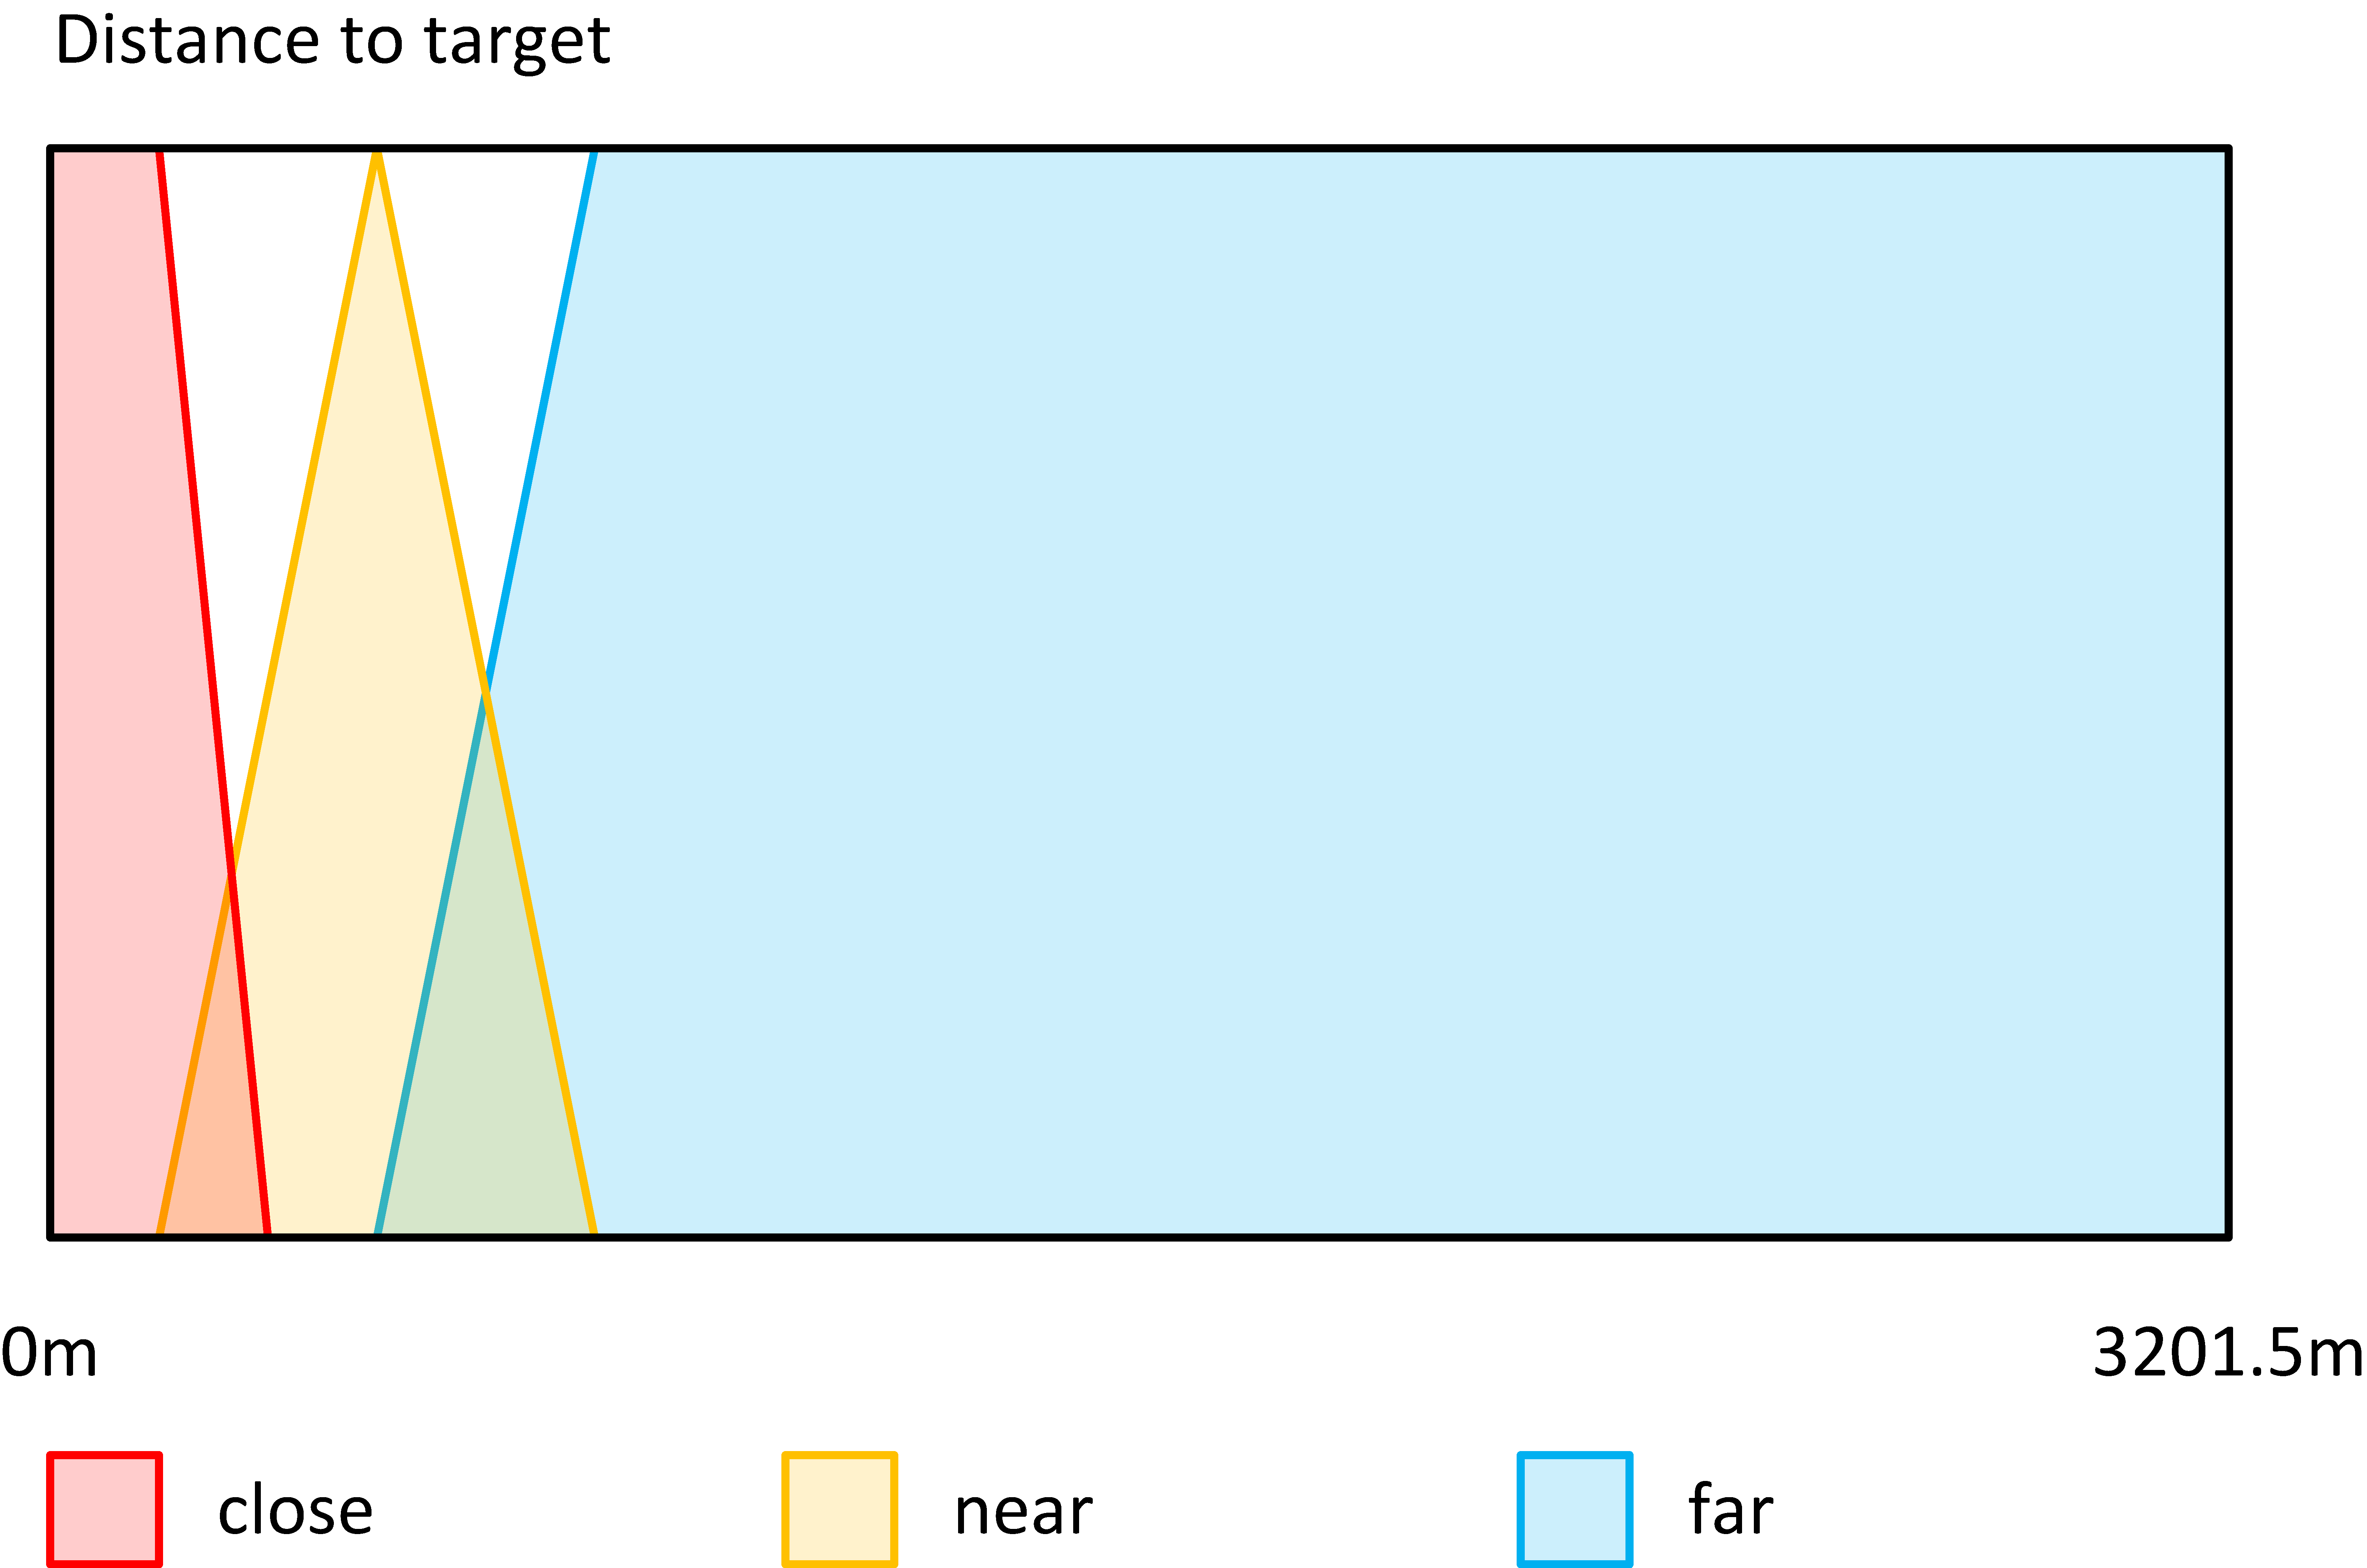
\includegraphics[scale=0.1]{./img/pdf/distanceSets.pdf}
\end{figure}

\subsubsection{Energy difference}

Energy difference is the difference between the saucer's energy and the opponent's energy. The universe of disclosure for energyDifference is between -10,000j to +10,000j, where 10,000j is the amount of energy that the saucers begin with. This linguistic variable determines who is winning, who is losing, or if the score is even. It is used as input to decide how much energy is committed in firing the weapon, as well as whether or not to turn into or away from the enemy. The following fuzzy sets are created for energy difference:

\begin{figure}[H]
\centering
\caption{Energy difference fuzzy sets}
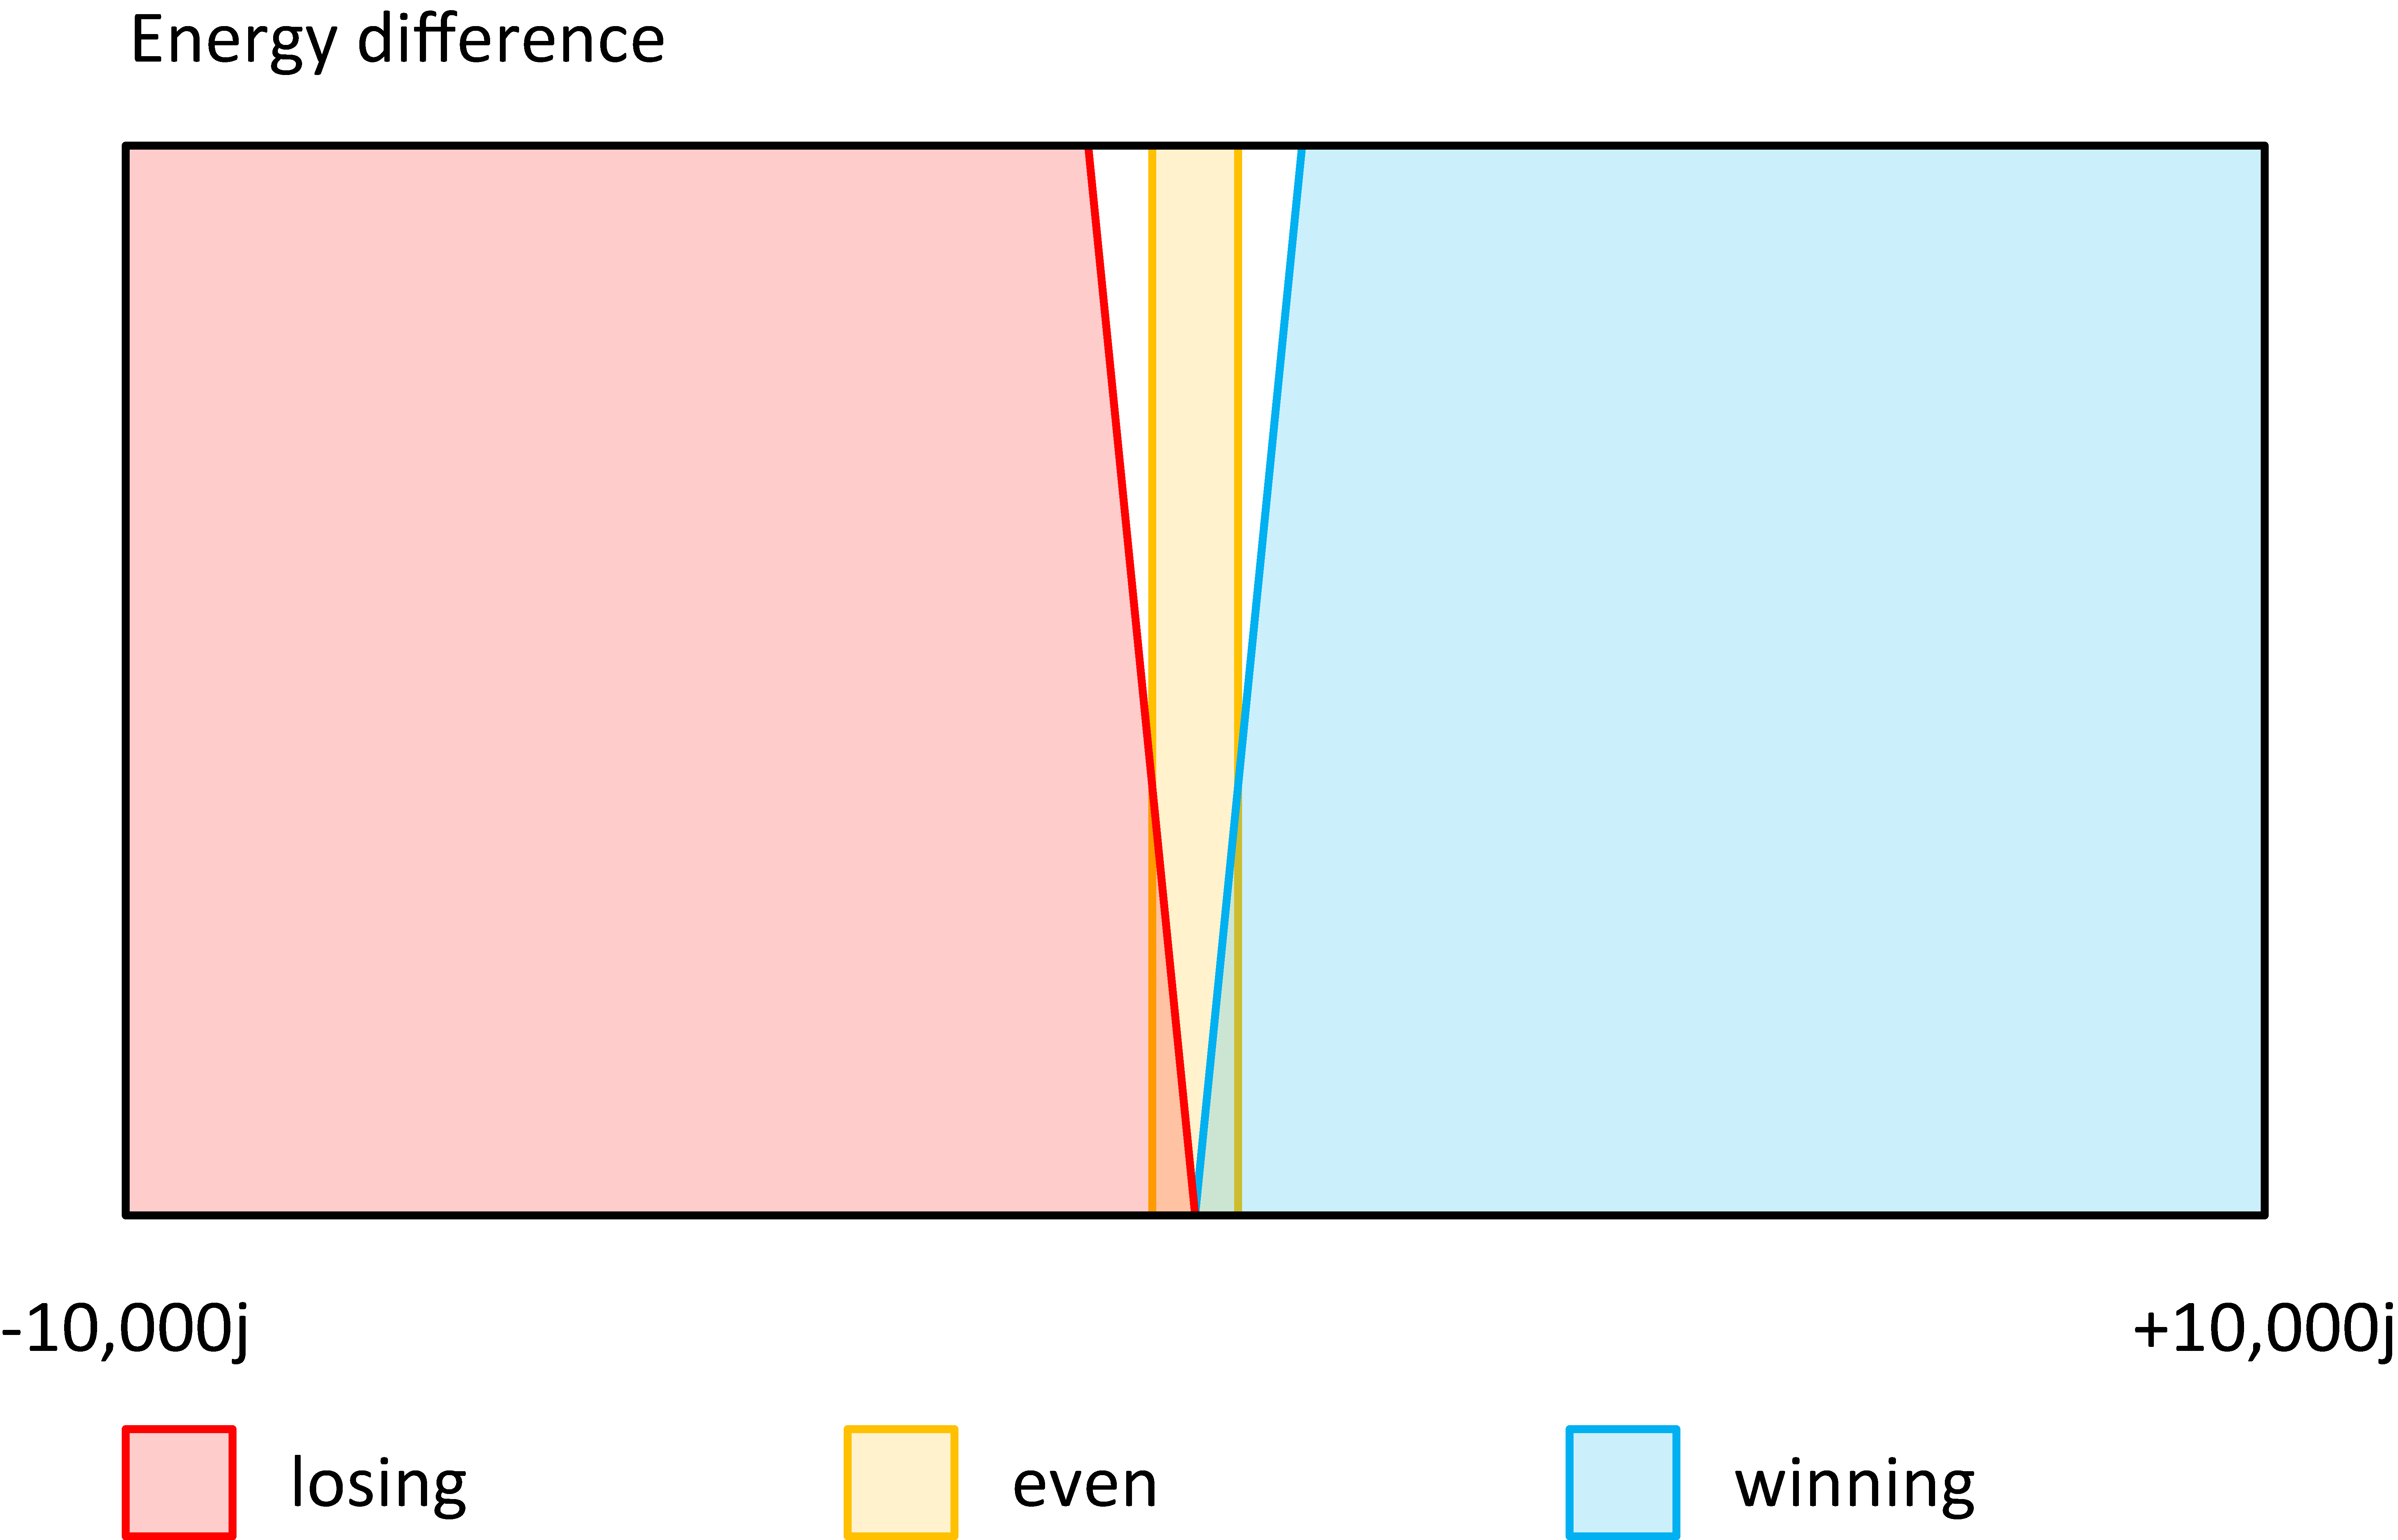
\includegraphics[scale=0.1]{./img/pdf/energyDiffSets.pdf}
\end{figure}

\subsubsection{Heading angle}

Heading angle is the direction of the opponent in relation to the saucer, in degrees. After printing \mintinline{java}{opponentDirection} during execution, it is assumed that the universe of disclosure for this linguistic variable is from -360$^{\circ}$ to +360$^{\circ}$. The variable, in conjunction with energy difference, dictates how the saucer will turn, and has been configured with the following fuzzy sets:

\begin{figure}[H]
\centering
\caption{Heading angle fuzzy sets}
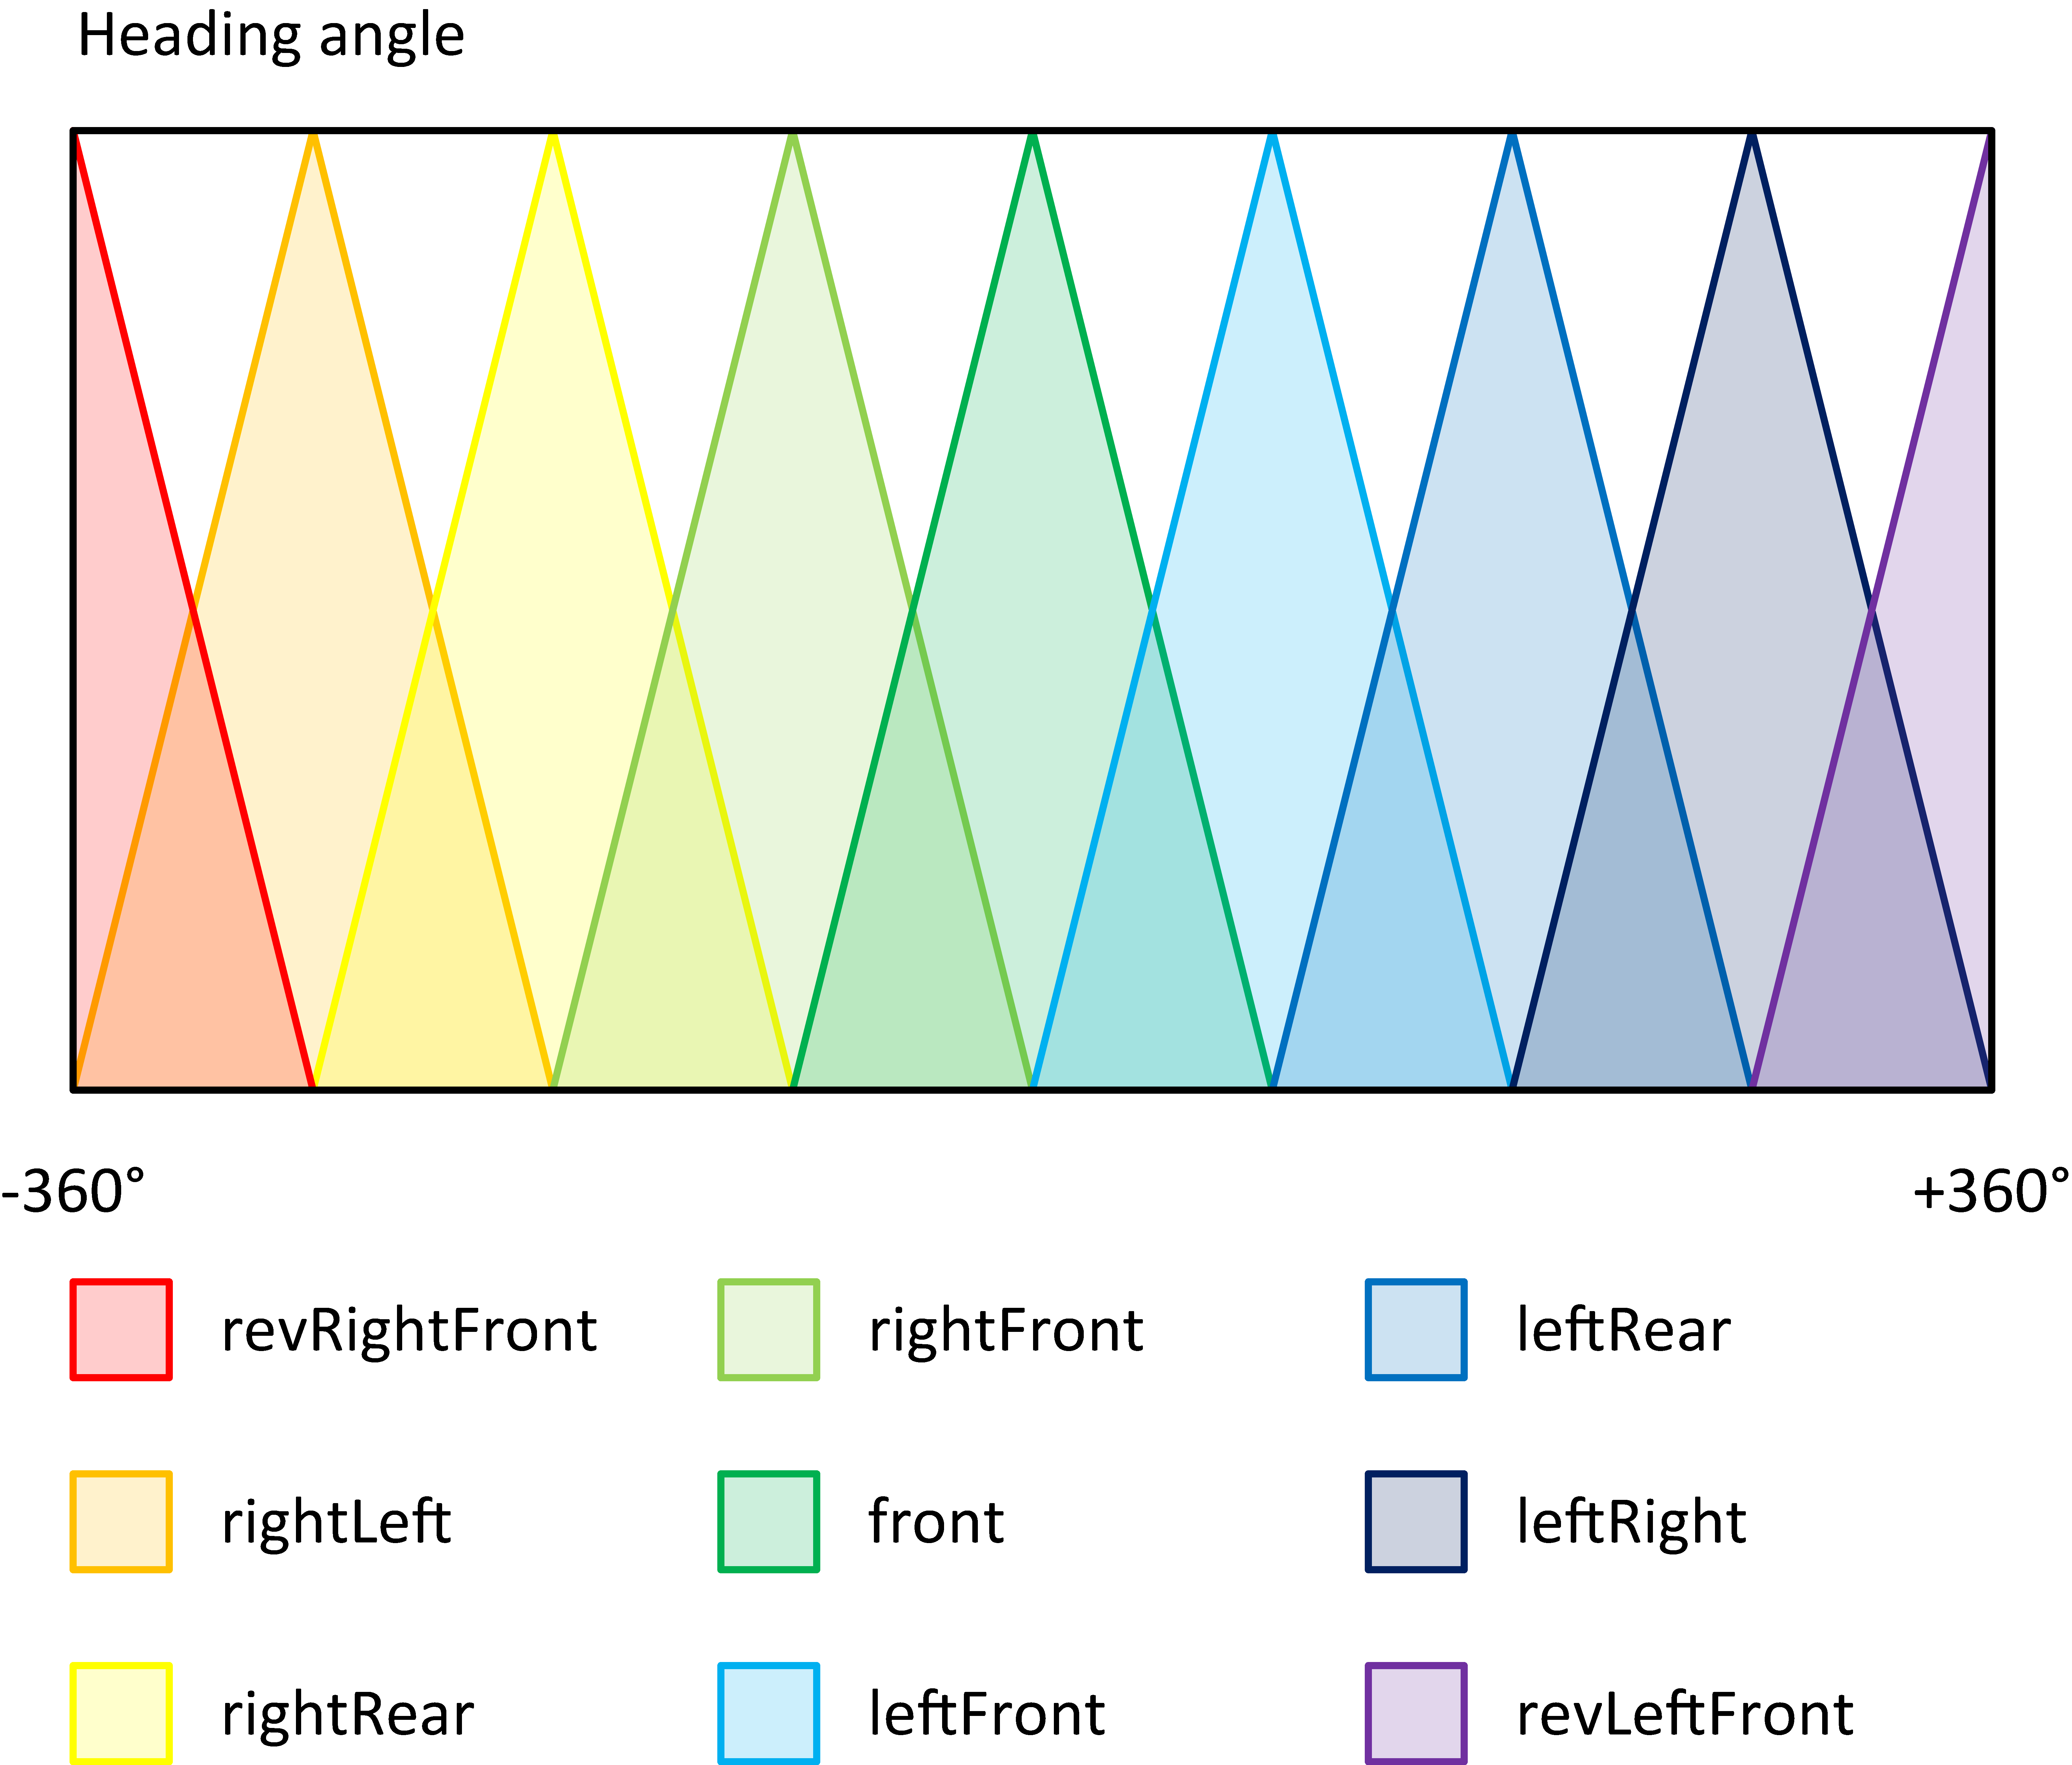
\includegraphics[scale=0.1]{./img/pdf/headingAngleSets.pdf}
\end{figure}

\subsection{Output variables}

\subsubsection{Turn}

The turn linguistic variable defines which heading the saucer will take, in degrees, according to the rules that govern turning. A zero value will turn towards the opponent, while 180$^{\circ}$ will turn away from the opponent and head into the opposite direction, turning left while doing so. A negative value will turn right, and a positive value will turn left. The linguistic variables used as input for the turning rules are energy difference and heading angle. See Table 1 for the turn rule table.

\begin{table}[H]
\centering
\caption{Turn rule table}
\label{Turn rule table}
\begin{tabular}{r|r|r|r}
 				& Losing 	& Even 		& Winning 	\\ \hline
revRightFront	& -180.0	& 0.0		& 0.0 		\\
rightLeft		& -90.0		& +90.0		& +90.0		\\
rightRear		& +180.0	& -180.0	& -180.0 	\\
rightFront		& +90.0		& -90.0 	& -90.0 	\\
front 			& -180.0	& 0.0 		& 0.0 		\\
leftFront 		& -90.0		& +90.0 	& +90.0		\\
leftRear 		& -180.0	& +180.0 	& +180.0 	\\
leftRight 		& +270.0	& -270.0 	& -270.0 	\\
revLeftFront 	& -180.0	& 0.0 		& 0.0 		\\
\end{tabular}
\end{table}

When winning or if the score is even, turn towards the enemy and commit to the engagement. Otherwise, if losing, turn away from the enemy and keep him at a relatively safe distance to minimize damage from cannon fire.
\\
\\
For example: IF (winning) AND (front) THEN (0.0)
\\
In other words, if winning and enemy is in front, then keep heading towards him.
\\
\\
In contrast: IF (losing) AND (front) THEN (-180.0)
\\
This will perform the opposite, and the saucer will turn right, into the opposite direction if the enemy is in front.

\subsubsection{Speed}

The speed linguistic variable defines how much energy to use for flight and is governed by rules which use distance and energy difference as inputs. See Table 2 for the speed rule table.

\begin{table}[H]
\centering
\caption{Speed rule table}
\label{Speed rule table}
\begin{tabular}{r|r|r|r}
 		& Losing & Even & Winning \\ \hline
Close	& 125.0 & 50.0 	& 50.0 \\
Near	& 100.0 & 50.0 	& 125.0 \\
Far		& 50.0 	& 100.0 & 125.0 \\
\end{tabular}
\end{table}

When winning, the strategy is as follows. If close or near, use the minimum speed to prevent overshooting the enemy, and also allow the enemy to overtake so that it can be followed. If near, use maximum speed to catch up to get within a more lethal range for the cannon.

When the score is even, the strategy is to be more conservative with energy and only used medium speed if far. Otherwise, use the minimum speed if close or near.

When losing, the strategy is to fly fast away from the enemy if close, and fly at a moderate speed if near. Otherwise use the minimum speed if far away.

\subsubsection{Firepower}

The firepower linguistic variable determines how much energy to use when firing the cannon, and is controlled by rules which use energy difference and distance as inputs. See Table 3 for the firepower rule table.

\begin{table}[H]
\centering
\caption{Firepower rule table}
\label{Firepower rule table}
\begin{tabular}{r|r|r|r}
 		& Losing 	& Even 		& Winning	\\ \hline
Close	& 50.0		& 50.0 		& 100.0		\\
Near	& 0.0 		& 100.0 	& 100.0		\\
Far		& 0.0 		& 0.0 		& 0.0		\\
\end{tabular}
\end{table}

When winning, and the enemy is close or near, fire the cannon using maximum power. Otherwise if the score is even, only fire the cannon at medium power when the enemy is close, or at maximum power when the enemy is near. This is to increase the chance that the cannot round will reach the target. Finally, if losing, do not fire the cannon at all at, unless at close range.